\documentclass[12pt]{article}
\usepackage[margin=2.5cm]{geometry}
\usepackage{enumerate}
\usepackage{amsfonts}
\usepackage{amsmath}
\usepackage{fancyhdr}
\usepackage{amsmath}
\usepackage{amssymb}
\usepackage{amsthm}
\usepackage{mdframed}
\usepackage{graphicx}
\usepackage{subcaption}
\usepackage{adjustbox}
\usepackage{listings}
\usepackage{xcolor}
\usepackage{booktabs}
\usepackage[utf]{kotex}
\usepackage{hyperref}

\definecolor{codegreen}{rgb}{0,0.6,0}
\definecolor{codegray}{rgb}{0.5,0.5,0.5}
\definecolor{codepurple}{rgb}{0.58,0,0.82}
\definecolor{backcolour}{rgb}{0.95,0.95,0.92}

\lstdefinestyle{mystyle}{
    backgroundcolor=\color{backcolour},
    commentstyle=\color{codegreen},
    keywordstyle=\color{magenta},
    numberstyle=\tiny\color{codegray},
    stringstyle=\color{codepurple},
    basicstyle=\ttfamily\footnotesize,
    breakatwhitespace=false,
    breaklines=true,
    captionpos=b,
    keepspaces=true,
    numbers=left,
    numbersep=5pt,
    showspaces=false,
    showstringspaces=false,
    showtabs=false,
    tabsize=1
}

\lstset{style=mystyle}

\pagestyle{fancy}
\renewcommand{\headrulewidth}{0.4pt}
\lhead{CSC 209}
\rhead{Review 7 Solution}

\begin{document}
\title{CSC 209 Review 7 Solution}
\maketitle

\bigskip

\section{Exercises}

\begin{enumerate}[1.]
    \item

    First, I need to justify if the folllowing declarations legal on an individual basis:

    \bigskip

    \texttt{struct \{int x, y;\} x;}

    \texttt{struct \{int x, y;\} y;}

    \bigskip

    The struct \texttt{struct \{int x, y;\} x;} is legal. \texttt{struct \{int x, y;\} x;}
    is equivalent to

\begin{lstlisting}[language=c]
    struct {
        int x;
        int y;
    } x;
\end{lstlisting}

    and `x' beside struct represents variable of that type. It is used to declare struct
    and access members of the struct (e.g. \texttt{x.x},, \texttt{x.y}).

    \bigskip

    The same is true for \texttt{struct \{int x, y;\} y;}.

    \bigskip

    Second, I need to answer if both declarations of struct can appear in a program.

    \bigskip

    The answer is yes. Each structure has a separate name space for it's members.

    \bigskip

    \underline{\textbf{Notes}}

    \begin{itemize}
        \item \textbf{Declaring Structure Variables}

        \begin{itemize}
            \item Struct can have many variables that represent the same struct

            \bigskip

            \begin{center}
            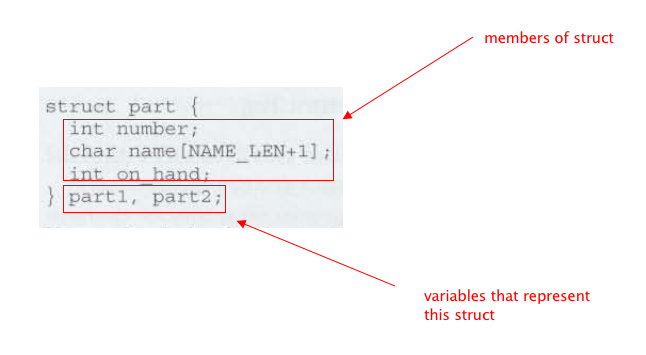
\includegraphics[width=0.8\linewidth]{images/review_7_solution_1.png}
            \end{center}
        \end{itemize}

        \bigskip

        \item \textbf{Initializing Structure Variables}

        \begin{itemize}
            \item Struct can be initialized with preset values (like python class under \_\_init\_\_)

            \bigskip

            \begin{center}
            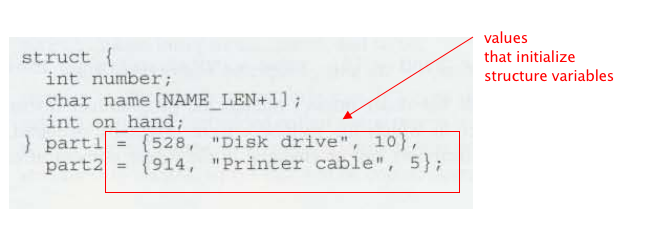
\includegraphics[width=0.8\linewidth]{images/review_7_solution_2.png}
            \end{center}

        \end{itemize}
    \end{itemize}

    \item

    \begin{enumerate}[a)]
        \item

        I need to declare structure variables named \texttt{c1}, \texttt{c2} and \texttt{c3},
        each having members \texttt{real} and \texttt{imaginary} of type \texttt{double}.

        \bigskip

        The solution to this problem is:

        \bigskip

\begin{lstlisting}[language=c]
    struct {
        double real, imaginary;
    } c1, c2, c3;
\end{lstlisting}

        \item

        I need to modify the declaration in part a) so that

        \begin{itemize}
            \item \texttt{c1}'s members initially have the values 0.0 and 1.0
            \item \texttt{c2}'s members initially have the values 1.0 and 0.0
            \item \texttt{c3} is not initialized
        \end{itemize}

        \bigskip

        The solution to this problem is:

        \bigskip

\begin{lstlisting}[language=c]
    struct {
        double real, imaginary;
    } c1 = {0.0, 1.0},
      c2 = {1.0, 0.0},
      c3;
\end{lstlisting}

        \bigskip

        \underline{\textbf{Notes}}

        \begin{itemize}
            \item \textbf{Designated Initializer}

            \begin{itemize}
                \item Allows specific member variable to be initialized
                \item Allows member variables to be initialized in any order
            \end{itemize}

            \bigskip

            \underline{\textbf{Example}}

            \bigskip

            \begin{center}
            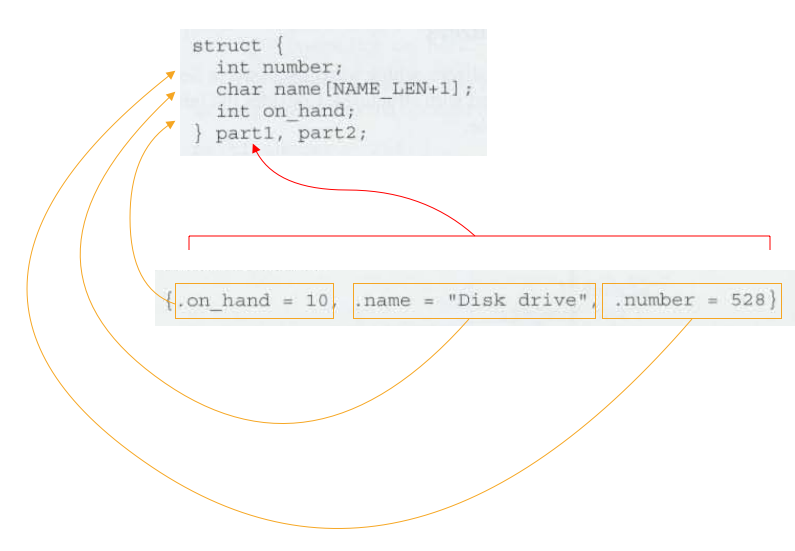
\includegraphics[width=0.8\linewidth]{images/review_7_solution_3.png}
            \end{center}
        \end{itemize}

        \item

        I need to write statements that copy the members of \texttt{c2} to \texttt{c1}.

        \bigskip

        Copying the members of \texttt{c2} and {c1} can be done in one statement.

        \bigskip

        Below is the solution to this problem:

        \bigskip

\begin{lstlisting}[language=c]
    c2 = c1
\end{lstlisting}

        \item

        I need to write statements that add the corresponding members of \texttt{c1}
        and \texttt{c2} and store the result in \texttt{c3}.

        \bigskip

        The solution to this problem is:


\begin{lstlisting}[language=c]
    struct {
        double real, imaginary;
    } c1 = {0.0, 1.0},
        c2 = {1.0, 0.0},
        c3;

    ...

    c3 = c1 + c2;
\end{lstlisting}

        \bigskip

        \underline{\textbf{Notes}}

        \begin{itemize}
            \item member variables of struct contains two operators \& and \texttt{.} (e.g \&\texttt{part1.number} and \texttt{part1.number})
            \item \& accesses memory address of the member variable, where as \texttt{.} accesses value
            \item \texttt{part1 = part2} \underline{copies} contents in \texttt{part2} to corresponding
            member variable in \texttt{part1}

            \bigskip

            \begin{center}
            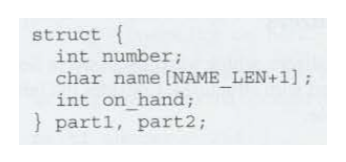
\includegraphics[width=0.5\linewidth]{images/review_7_solution_4.png}
            \end{center}
        \end{itemize}

    \end{enumerate}

    \item

    \begin{enumerate}[a)]
        \item

        I need to declare a tag named \texttt{complex} for a structure with two members
        \texttt{real} and \texttt{imaginary}, of type \texttt{double}

        \bigskip

        The solution to this problem is:

        \bigskip

\begin{lstlisting}[language=c]
    struct complex {
        double real, imaginary;
    };
\end{lstlisting}


        \underline{\textbf{Notes}}

        \begin{itemize}
            \item \textbf{Declaring a Structure Tag}

            \begin{itemize}
                \item allows to use struct in function calls
                \item allows to use the same struct in multiple files of a program
            \end{itemize}

            \bigskip

            \begin{center}
            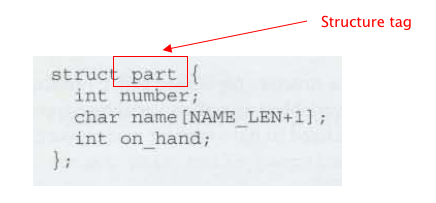
\includegraphics[width=0.6\linewidth]{images/review_7_solution_5.png}
            \end{center}
        \end{itemize}

        \item

        I need to use the \texttt{complex} tag to declare variables named \texttt{c1},
        \texttt{c2}, \texttt{c3}.

        \bigskip

        The solution to this problem is:

        \bigskip

\begin{lstlisting}[language=c]
    struct complex {
        double real, imaginary;
    } c1, c2, c3;
\end{lstlisting}

        \item

        I need to write a function named \texttt{make\_complex} that satisfies the following:

        \begin{itemize}
            \item The function \texttt{make\_complex} should have two parameters (\texttt{real}, \texttt{imaginary}) of type \texttt{double}
            \item The function \texttt{make\_complex} should store the two arguments in \texttt{complex} struct
            \item The function \texttt{make\_complex} should return the struct
        \end{itemize}

        \bigskip

        The solution to this problem is:

        \bigskip

\begin{lstlisting}[language=c]
    struct complex {
        double real, imaginary;
    };

    struct complex (double real, double imaginary) {
        struct complex c1;

        c1.real = real;
        c1.imaginary = imaginary;

        return c1;
    }
\end{lstlisting}

        \bigskip

        \underline{\textbf{Notes}}

        \begin{itemize}
            \item \textbf{Declaring Variables Cont.}

            \begin{itemize}
                \item Once the struct tag is formed, it can be used to declare variables

                \bigskip

                \underline{\textbf{Example}}

                \bigskip

                \texttt{struct part part1, part2}

                \bigskip

                \item Structure tag can be combined with the declaration of structure variables.
                \begin{itemize}
                    \item it's like creating a global variable (if it's outside of main), or local
                    variable (if it's created inside a function) at the instant the struct is formed
                \end{itemize}

                \bigskip

                \begin{center}
                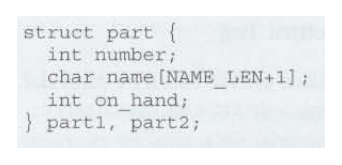
\includegraphics[width=0.6\linewidth]{images/review_7_solution_6.png}
                \end{center}

                \item Declared variables can set values the moment it's declared

                \bigskip

                \underline{\textbf{Example}}

                \bigskip

                \texttt{struct part part1 = \{528, "Disk Drive", 10\}}
            \end{itemize}
        \end{itemize}

        \item

        I need to write a function named \texttt{add\_complex} that satisfies the following:

        \begin{itemize}
            \item The function \texttt{add\_complex} should have 2 parameters of type \texttt{struct complex}
            \item The function \texttt{add\_complex} should add the corresponding members of its arguments
            \item The function \texttt{add\_complex} should return the result of type \texttt{struct complex}
        \end{itemize}

        \bigskip

        The solution to this problem is:

        \bigskip

\begin{lstlisting}[language=c]
    struct complex {
        double real, imaginary;
    };

    struct complex add_complex (struct complex c1, struct complex c2) {
        struct complex c3;

        c3.real = c1.real + c2.real;
        c3.imaginary = c1.imaginary + c2.imaginary;

        return c3;
    }
\end{lstlisting}
    \end{enumerate}

    \item

    I need to repeat exercise 3 but using a \texttt{type} named \texttt{complex}.

    \bigskip

    \begin{enumerate}[a)]
        \item

\begin{lstlisting}[language=c]
    typedef struct {
        double real, imaginary;
    } Complex;
\end{lstlisting}

        \item

\begin{lstlisting}[language=c]
    typedef struct {
        double real, imaginary;
    } Complex;

    ...

    Complex c1, c2, c3;
\end{lstlisting}

        \item

\begin{lstlisting}[language=c]
    typedef struct {
        double real, imaginary;
    } Complex;

    Complex make_complex(double real, double imaginary) {
        Complex c;

        c.real = real;
        c.imaginary = imaginary;

        return c;
    }
\end{lstlisting}

        \item

\begin{lstlisting}[language=c]
    typedef struct {
        double real, imaginary;
    } Complex;

    Complex add_complex(Complex c1, Complex c2) {
        Complex c3;

        c3.real = c1.real + c2.real;
        c3.imaginary = c1.imaginary + c2.imaginary;

        return c3;
    }
\end{lstlisting}
    \end{enumerate}

    \underline{\textbf{Notes}}

    \begin{itemize}
        \item \textbf{Structure Type}

        \begin{itemize}
            \item Is an alternative to declaring a structure tag

            \bigskip

            \begin{center}
            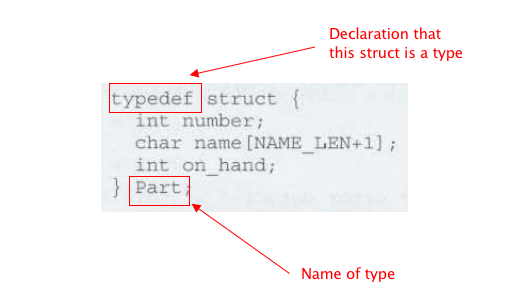
\includegraphics[width=0.5\linewidth]{images/review_7_solution_7.png}
            \end{center}

            \item Allows us to define a genuine type name

            \bigskip

            \underline{\textbf{Example}}

            \bigskip

            \texttt{Part part1, part2;}
            \item Once declared, cannot define a structure tag with the same name
        \end{itemize}
    \end{itemize}

    \item

    \begin{enumerate}[a)]
        \item

        I need to write the following function

        \bigskip

        \texttt{int day\_of\_year (struct date d);}

        \bigskip

        satisfying the following requirements:

        \begin{itemize}
            \item The \texttt{date} structure should contain three members: \texttt{month},
            \texttt{day}, and \texttt{year} all of type \texttt{int}

            \item The function \texttt{day\_of\_year} should return the day of the year (an integer between 1 and 366)
            that corresponds to the date \texttt{d}
        \end{itemize}

        \bigskip

        The solution to this problem is:

        \bigskip

\begin{lstlisting}[language=c]

    struct date {
        int month, day, year;
    };

    int day_of_year (struct date d);

    ...

    int day_of_year (struct date d) {
        bool leap_year = false;
        int days = 0, days_in_month[] = {
            31, 28, 31, 30,
            31, 30, 31, 31,
            30, 31, 30, 31};

        // check if it's the leap year
        if (((d.year % 4 == 0) &&
            (d.year % 100 != 0)) ||
            (d.year % 400 == 0)) {

                leap_year = true;
            }


        // add days from months
        for (int i = 0; i < d.month; i++) {
            if (i == d.month-1) {
                days += d.day;
                continue;
            }

            days += days_in_month[i];
        }


        // add 1 more day if month > 2 and it's leap year
        if (leap_year && d.month > 2) {
            days += 1;
        }


        // return days
        return days;
    }
\end{lstlisting}

        \item

        I need to write the following function

        \bigskip

        \texttt{int compare\_dates (struct date d1, struct date d2);}

        \bigskip

        satisfying the following requirements:

        \begin{itemize}
            \item The function \texttt{compare\_dates} should return
            \begin{itemize}
                \item -1 if \texttt{d1} is an earlier date than \texttt{d2}
                \item +1 if \texttt{d1} is a later date than \texttt{d2}
                \item 0 if \texttt{d1} and \texttt{d2} are the same
            \end{itemize}
        \end{itemize}

        \bigskip

        The solution to this problem is:

\begin{lstlisting}[language=c]
    #include <stdio.h>
    #include <string.h>
    #include <stdbool.h>

    struct date {
        int month, day, year;
    };

    ...

    int compare_dates (struct date d1, struct date d2) {
        char s1[9], s2[9];

        sprintf(s1,"%4d%2d%2d", d1.year, d1.month, d1.day);
        sprintf(s2,"%4d%2d%2d", d2.year, d2.month, d2.day);

        // return days
        return strcmp(s1,s2);
    }
\end{lstlisting}
    \end{enumerate}

    \item

    I need to write the following function

    \bigskip

    \texttt{struct time split\_time(long total\_seconds)}

    \bigskip

    satisfying the following requirements:

    \begin{itemize}
        \item The \texttt{time} structure has three members \texttt{hours}, \texttt{minutes}, \texttt{seconds}
        \item The function \texttt{split\_time} should return \texttt{time} struct containing
        equivalent time in \texttt{hours} (0-23), \texttt{minutes} (0-59), \texttt{seconds} (0-59)
    \end{itemize}

    \bigskip

    The solution to this problem is:

\begin{lstlisting}[language=c]
    #include <stdio.h>
    #include <string.h>
    #include <stdbool.h>

    struct time {
        int hours, minutes, seconds;
    };

    struct time split_time (long total_seconds);

    ...

    struct time split_time (long total_seconds) {
        struct time t;
        int s = (int)total_seconds;

        printf("%d\n", s);

        t.hours = s / 3600;
        s = s - (t.hours * 3600);

        t.minutes = s / 60;
        s = s - (t.minutes * 60);

        t.seconds = s;

        return t;
    }
\end{lstlisting}

    \item

    \begin{enumerate}[a)]
        \item

        I need to write a function that satisfies the following requirements:

        \begin{itemize}
            \item The function should reduce the fraction \texttt{f} to lowest terms
            \item The struct \texttt{fraction} contains two members: \texttt{numberator} and \texttt{denominator}, and
            both are type \texttt{int}
        \end{itemize}

        \bigskip

        The solution to this problem is:

        \bigskip

\begin{lstlisting}[language=c]
    struct fraction {
        int numerator, denominator;
    };

    ...

    struct fraction reduce (struct fraction f) {

        int gcd;

        struct fraction f2;

        if (f.numerator >= f.denominator) {
            gcd = f.denominator;
        } else {
            gcd = f.numerator;
        }

        while (gcd > 0) {
            if ((f.numerator % gcd == 0) &&
                (f.denominator % gcd == 0)) {
                break;
            }

            gcd--;
        }

        f2.denominator = f.denominator/gcd;
        f2.numerator = f.numerator/gcd;

        return f2;
    }
\end{lstlisting}

        \item

        I need to write a function that adds two fractions \texttt{f1} and \texttt{f2}.

        \bigskip

        The solution to this problem is:

\begin{lstlisting}[language=c]
    struct fraction {
        int numerator, denominator;
    };

    ...

    struct fraction add (struct fraction *f1, struct fraction *f2) {

        struct fraction f3;

        if (f1->denominator != f2->denominator) {
            f3.numerator = (f1->numerator * f2->denominator) + (f2->numerator * f1->denominator);
            f3.denominator = f1->denominator * f2->denominator;
        } else {
            f3.numerator = f2->numerator + f1->numerator;
        }

        f3 = reduce(f3);

        return f3;
    }
\end{lstlisting}

        \item

        I need to create a function that subtracts two fractions \texttt{f1} and \texttt{f2}.

        \bigskip

        The solution to this problem is:

\begin{lstlisting}[language=c]
    struct fraction {
        int numerator, denominator;
    };

    ...

    struct fraction subtract (struct fraction *f1, struct fraction *f2) {

        struct fraction f3;

        if (f1->denominator != f2->denominator) {
            f3.numerator = (f2->numerator * f1->denominator) - (f1->numerator * f2->denominator);
            f3.denominator = f1->denominator * f2->denominator;
        } else {
            f3.numerator = f2->numerator - f1->denominator;
        }

        f3 = reduce(f3);

        return f3;
    }
\end{lstlisting}

        \item

        I need to create a function that divides fractions \texttt{f1} by fraction \texttt{f2}.

        \bigskip

        The solution to this problem is:

\begin{lstlisting}[language=c]
    struct fraction {
        int numerator, denominator;
    };

    ...

    struct fraction divide (struct fraction *f1, struct fraction *f2) {

        struct fraction f3;

        f3.denominator = f1->denominator * f2->numerator;
        f3.numerator = f1->numerator * f2->denominator;

        f3 = reduce(f3);

        return f3;
    }


\end{lstlisting}

    \end{enumerate}

    \item

    \begin{enumerate}[a)]
        \item

        I need to write a declaration for a \texttt{const} variable named \texttt{MAGNETA}
        of type \texttt{struct color} that satisfies the following

        \begin{itemize}
            \item \texttt{red} has value 255
            \item \texttt{green} has value 0
            \item \texttt{blue} has value 255
        \end{itemize}

        \bigskip

        The solution to this problem is:

\begin{lstlisting}[language=c]
    struct color {
        int red;
        int green;
        int blue;
    };

    const struct color MAGNETA = {255, 0, 255}
\end{lstlisting}
        \item

        I need to rewrite above to use a designated initializer that doesn't specify the value
        of \texttt{green}.

        \bigskip

        The solution to this problem is:

\begin{lstlisting}[language=c]
    struct color {
        int red;
        int green;
        int blue;
    };

    const struct color MAGNETA = {.red = 255, .blue = 255};
\end{lstlisting}

        \bigskip

        \underline{\textbf{Notes}}

        \begin{itemize}
            \item \texttt{int} variable prints 0, if nothing is in it
        \end{itemize}
    \end{enumerate}

    \item

    \begin{enumerate}[a)]
        \item

        I need to write the function

        \bigskip

        \texttt{struct color make\_color(int red, int green, int blue)}

        \bigskip

        that satisfies the following requirements:

        \begin{itemize}
            \item The function \texttt{make\_color} should return \texttt{color} structure
            \item The function \texttt{make\_color} should return 0 for a member variable if the corresponding argument has value less than 0
            \item The function \texttt{make\_color} should return 255 for a member variable if the corresponding argument has value greater than 255
        \end{itemize}

        \bigskip

        The solution to this problem is:

\begin{lstlisting}[language=c]
    struct color make_color(int red, int green, int blue) {
        struct color c;

        red = red < 0 ? 0 : red;
        green = green < 0 ? 0 : green;
        blue = blue < 0 ? 0 : blue;

        red = red > 255 ? 255 : red;
        blue = blue > 255 ? 255 : blue;
        green = green > 255 ? 255 : green;

        c.red = red;
        c.green = green;
        c.blue = blue;

        return c;
    }
\end{lstlisting}

        \item

        I need to write the function

        \bigskip

        \texttt{int getRed(struct color c)}

        \bigskip

        that returns the value of \texttt{c}'s red member.

        \bigskip

        The solution to this problem is

\begin{lstlisting}[language=c]
    int getRed(struct color c) {
        return c.red;
    }
\end{lstlisting}

        \item

        I need to write the function

        \bigskip

        \texttt{bool equal\_color(struct color color1, struct color color2)}

        \bigskip

        satisfying the following requirement

        \begin{itemize}
            \item The function \texttt{equal\_color} returns true if the corresponding members of
            \texttt{color1} and \texttt{color2} are equal
        \end{itemize}

        \bigskip

        The solution to this problem is:

        \bigskip

\begin{lstlisting}[language=c]
    bool equal_color(struct color color1, struct color color2) {
        if ((color1.red == color2.red) &&
            (color1.green == color2.green) &&
            (color1.blue == color2.blue)) {
            return true;
        }

        return false;
    }
\end{lstlisting}

        \item

        I need to write the function

        \bigskip

        \texttt{struct color brighter(struct color c)}

        \bigskip

        satisfying the following requirement

        \begin{itemize}
            \item if all members of \texttt{c} are zero, then return color whose all
            members have value 3
            \item If any member of \texttt{c} is greater than 0 but less than 3, it is replaced
            by 3 before the division by 0.7
            \item if any member of \texttt{c} is greater than equal to 3, than, divide by 0.7
            \item if diving by 0.7 exceeds 255, then replace it with 255
        \end{itemize}

        \bigskip

        The solution to this problem is:

        \bigskip

\begin{lstlisting}[language=c]
    struct color brighter(struct color c) {

        if((c.red == 0 ) &&
            (c.green == 0) &&
            (c.blue == 0)) {

            c.red = 3;
            c.green = 3;
            c.blue = 3;

            return c;
        }

        c.red = c.red < 3 && c.red > 0 ? 3 : c.red;
        c.green = c.green < 3 && c.green > 0 ? 3 : c.green;
        c.blue = c.blue < 3 && c.blue > 0 ? 3 : c.blue;

        c.red = (int)(c.red/0.7);
        c.green = (int)(c.green/0.7);
        c.blue = (int)(c.blue/0.7);

        c.red = c.red > 255 ? 255 : c.red;
        c.green = c.green > 255 ? 255 : c.green;
        c.blue = c.blue > 255 ? 255 : c.blue;

        return c;
    }
\end{lstlisting}

        \item

\begin{lstlisting}[language=c]
    struct color darker(struct color c) {

        if((c.red == 0 ) &&
            (c.green == 0) &&
            (c.blue == 0)) {

            c.red = 3;
            c.green = 3;
            c.blue = 3;

            return c;
        }

        c.red = c.red < 3 && c.red > 0 ? 3 : c.red;
        c.green = c.green < 3 && c.green > 0 ? 3 : c.green;
        c.blue = c.blue < 3 && c.blue > 0 ? 3 : c.blue;

        c.red = (int)(c.red*0.7);
        c.green = (int)(c.green*0.7);
        c.blue = (int)(c.blue*0.7);

        c.red = c.red > 255 ? 255 : c.red;
        c.green = c.green > 255 ? 255 : c.green;
        c.blue = c.blue > 255 ? 255 : c.blue;

        return c;
    }
\end{lstlisting}

    \end{enumerate}

    \item

    \bigskip

    \begin{enumerate}[a)]

        \item

\begin{lstlisting}[language=c]
    int area(struct rectangle r) {
        return ((r.upper_left.y - r.lower_right.y) *
                (r.lower_right.x - r.upper_left.x));
    }
\end{lstlisting}

        \bigskip

        \underline{\textbf{Notes}}

        \begin{itemize}
            \item \textbf{Nested Structure}

            \begin{itemize}
                \item Works just like a nested class

                \bigskip

                \begin{center}
                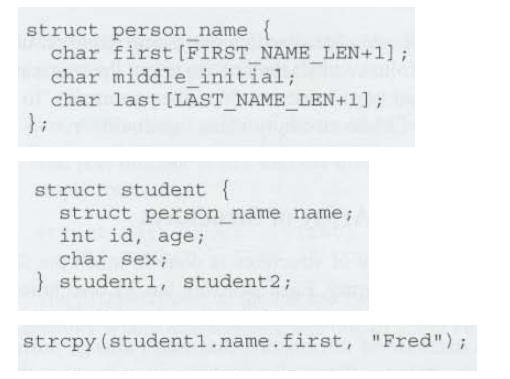
\includegraphics[width=0.8\linewidth]{images/review_7_solution_8.png}
                \end{center}
            \end{itemize}
        \end{itemize}

        \item

\begin{lstlisting}[language=c]
    struct point center(struct rectangle r) {
        struct point pt;

        pt.x = (int)((r.upper_left.y - r.lower_right.y)/2);
        pt.y = (int)((r.lower_right.x - r.upper_left.x)/2);

        return pt;
    }
\end{lstlisting}

        \item

\begin{lstlisting}[language=c]
    struct rectangle translate(struct rectangle r, int x, int y) {

        r.upper_left.x += x;
        r.upper_left.y += y;

        r.lower_right.x += x;
        r.lower_right.y += y;

        return r;
    }
\end{lstlisting}

        \item

\begin{lstlisting}[language=c]
    bool inside_rectangle(struct rectangle r, struct point p) {
        if ((p.x > r.upper_left.x && p.x < r.lower_right.x) &&
            (p.y > r.lower_right.y && p.y < r.upper_left.y)) {
                return true;
            }

        return false;
    }
\end{lstlisting}

    \end{enumerate}

\end{enumerate}

\end{document}